\documentclass[conference]{IEEEtran}
\usepackage{amsmath,amssymb,booktabs,graphicx,balance}
\usepackage[hidelinks]{hyperref}
\usepackage{iftex}
\ifXeTeX
\usepackage{fontspec}
\setmainfont{texgyretermes-regular.otf}[BoldFont=texgyretermes-bold.otf,ItalicFont=texgyretermes-italic.otf,BoldItalicFont=texgyretermes-bolditalic.otf]
\setsansfont{texgyreheros-regular.otf}[BoldFont=texgyreheros-bold.otf,ItalicFont=texgyreheros-italic.otf]
\setmonofont{texgyrecursor-regular.otf}[BoldFont=texgyrecursor-bold.otf]
\fi
\title{Sharing Retained Git Events in a Graph Memory for Coding Agents}
\author{\IEEEauthorblockN{Anonymous working draft}}
\begin{document}
\maketitle
\begin{abstract}
A coding agent that knows one file involved in a change can consult prior co-edits to find another file worth reading. A small memory can retain a multi-file commit on behalf of several paths. When one path evicts its reference, another may still hold the original evidence. We demonstrate an event store in which visitors can inspect who retained an event, follow its contribution to a score and compare the resulting file recommendations. An exact SQLite reader partitions the history into retained and fully evicted events. On 196 queries from three long Git histories it returned the same eight file IDs and scores as full reconstruction while transferring 27,716 bytes of event payload from SQLite, against 358,964 for a packed full-history reader. Without archive access, broadening the read increased Recall@8 from 41.97\% to 43.53\% and nearly quadrupled the number of events decoded. A separate transfer experiment on Agent Retrieval Bench yielded an inconclusive 0.63-point difference in Recall@5. The demonstration exposes these costs and the cases in which more evidence displaces a relevant file.
\end{abstract}

\section{Who still holds the evidence?}
Suppose a coding agent opens a graph generator and wants the test that changes with it. The last eight commits touching the generator contain evidence about widely used graph utilities. Older fixes tied the generator to its test. The generator may have exhausted its memory budget while its less frequently modified test still retains the same old commits. A database that shares the immutable commit across participants can answer two different questions. What did the generator itself keep? Which surviving events still mention the generator?

Predicting companion changes from version histories has a long precedent in ROSE~\cite{zimmermann}. TAPE~\cite{tape} organizes temporal evidence for personal agents in a graph, and MemTrace~\cite{memtrace} checks the validity of restored evidence for coding agents. Our question concerns the relationship between who keeps an event, who can subsequently read it and what a complete answer costs. Every extra vote in our demonstration points to an observed commit. The inputs consist of successive changed paths and revision identifiers. The history ranker requires no file contents, repository-wide embeddings or static dependency graph.

\begin{figure}[t]
\centering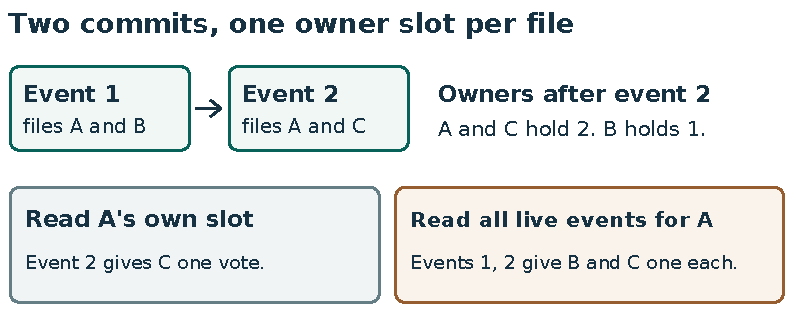
\includegraphics[width=\columnwidth]{retention.pdf}
\caption{The retention rule in a minimal example. After A's slot is overwritten, B still owns event 1. An incidence lookup from A can now explain its historical link to B.}
\label{fig:retention}
\end{figure}

Our interface lets visitors inspect opposing outcomes on two actual NetworkX commits, expand the evidence that determined the ranking, and compare it with an independently reconstructed Git projection. A companion console from our preceding prototype illustrates withdrawal and historical reads on a tool trace. Together the interfaces distinguish a change in the visible evidence, a change in the resulting rank and a change in whether the file actually helps the task.

\section{Storage and read contracts}
\subsection{Write one immutable event}
An accepted event $e$ has a monotonically increasing ID, a commit SHA and the distinct Python paths $M_e$ changed by that commit. Each path gets a stable integer ID at first appearance. Events with 2--64 paths enter the co-edit store. Single-file commits can still contribute to the frequency used to break ties. At time $t$, file $f$ owns its latest $b$ incident events $O_t(f)$, with $b=8$ in our primary experiments. Define the hot set
\[
 H_t=\bigcup_f O_t(f),\qquad I_t(a)=\{e\in H_t:a\in M_e\}.
\]
On insert, each member advances its queue. The event stays hot until its final owner releases it. The supporting structure maps an incident file to all live event IDs containing it. Each event body is stored once in the durable journal. Direct pair materialization for $m$ participating files would update $m(m-1)$ directed pair counts. Event admission adds $m$ incidences and can trigger separate eviction work for older events. The number of owner references is at most $b$ per file. The union, incidence index and durable archive have separate space costs.

\subsection{Rank paths or reconstruct the full answer}
Given a known anchor $a$, choose a set $E$ of events involving it. For each previously observed candidate $x\ne a$, compute $s(x)=\sum_{e\in E}{\bf 1}[x\in M_e]$. Rank by decreasing $s$, decreasing frequency in the preceding 32 commits and increasing first-seen ID. The owner-only reader uses $O_t(a)$. The shared reader uses $I_t(a)$ on the same retained events and access index. The latter may decode more event bodies. A third reader orders the eligible events by member count, breaking ties by recency, and decodes the smallest $b$. Finding these events requires inspecting their metadata.

A fourth contract requires the precise ordered IDs \emph{and scores} that all accepted history would produce. Since the live and evicted sets partition the history, the exact reader adds the votes from $I_t(a)$ to those from fully evicted events incident to $a$. Every co-edit contributes once. Ties and zero scores use the same order as the full reader. The full-history baseline retrieves event bodies by anchor with one indexed SQL statement and counts votes in the client. A materialized pair table and a direct full-count reference are additional controls.

One can sometimes certify an exact answer from the hot store. Let $D$ be the number of fully evicted events, $d_f$ the number involving $f$, and $v$ the number of visible joint events for $a,x$. The unknown sets for these paths lie in the same universe of $D$ events, giving
\[
v+\max(0,d_a+d_x-D)\ \le\ s_{\rm full}(x)\
\le\ v+\min(d_a,d_x).
\]
The lower bound follows by inclusion--exclusion, the upper by containment in either missing set. For example, if $D=3$, $d_a=2$ and $d_x=2$, at least one co-edit is already implied. For a ranked certificate we require fixed counts for the winning entries and upper keys that cannot displace them under the specified tie order. The analytical evaluator can request exact unresolved pair counts. The timed SQLite plan uses the simpler test $d_a=0$ and otherwise reads the missing events for the anchor.

\subsection{Durability and restart}
The SQLite implementation appends each event body and revision once in a transaction. A live table stores the IDs of events with a current owner. When the final owner releases an event, its members enter a cold posting index. A small directory identifies paths with cold postings. The hot reader holds both the owner queues and the incidence index in RAM. On reopening, it reads the directory and replays the live events in timestamp order. This reconstructs the queues because every path's last $b$ events belong to their union. The exact read then performs at most one archive query. The archive grows with accepted history. A finite cold-storage retention rule would change the full-history contract.

In a fault-injection test the writer rejected colliding retries and gaps, accepted identical retries, and rolled back a failed SQL transaction. Reopening midstream and appending further events preserved the independently calculated ranked outputs. We tested a single writer and public, append-only Git history. Changing an old event in place or processing concurrent branches requires an additional identity and consistency policy.

\begin{figure*}[t]
\centering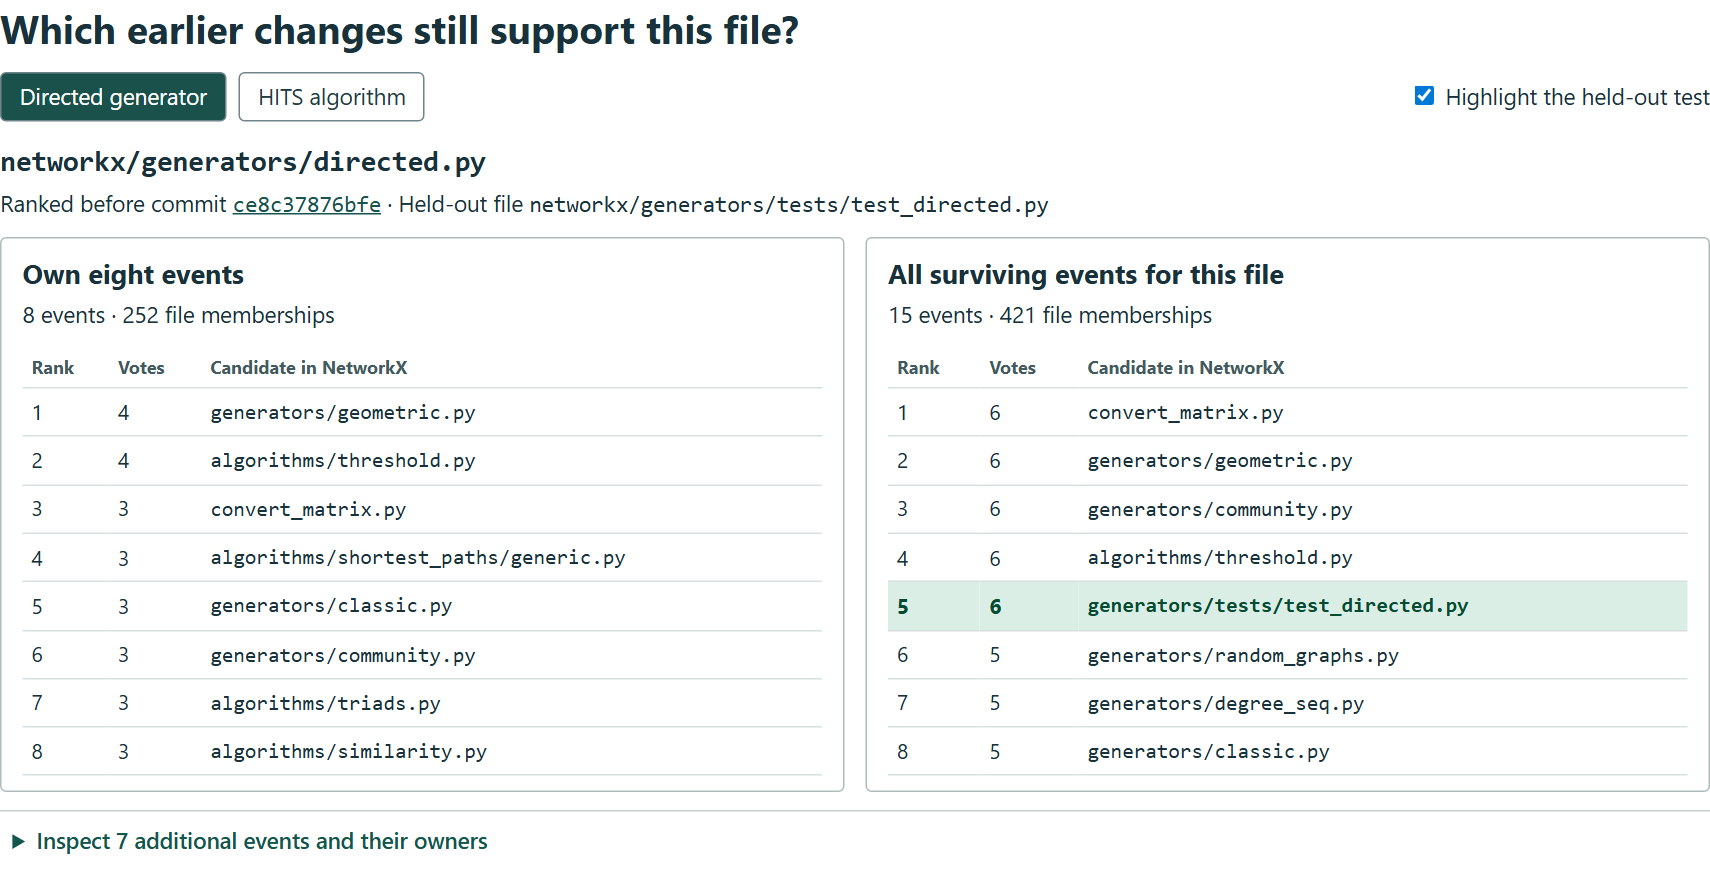
\includegraphics[width=.97\textwidth]{networkx-replay.png}
\caption{The English replay before NetworkX commit \texttt{ce8c3787}. Both views read the same retained store. Visitors can switch cases, hide the held-out annotation or expand the list of new witnesses to inspect their owners and source commits. The offline page embeds ranks computed from the Git prefix.}
\label{fig:networkx}
\end{figure*}

\section{Demonstration scenarios}
\subsection{Follow a winning historical link}
Open \texttt{replay.html} and choose the directed generator (Fig.~\ref{fig:networkx}). The query reveals the module \texttt{directed.py} immediately before NetworkX commit \texttt{ce8c3787}. Both tables use the same information available before the displayed commit. Each row shows a file's rank and number of co-edits. A check mark identifies the held-out test after ranking. Open the list of supporting events to see commit IDs and files that retained them.

The left-hand table reads eight events with 252 memberships. The right-hand table reads 15 with 421 memberships. Four of the additional events mention \texttt{test\_directed.py}. Its score rises to six, placing it fifth (Table~\ref{tab:demo}). One of those events, \texttt{539ad536}, is still held by the test itself. A visitor can follow the event back to the original patch. The page remains usable offline from the recorded projection.

\begin{table}[t]
\caption{Actions visible in the NetworkX replay. A rank outside the displayed eight is marked out. The participant counts measure work done before the held-out test is inspected.}
\label{tab:demo}\centering\small
\begin{tabular}{@{}llrrr@{}}\toprule
Known file & Read policy & Events & Members & Test rank\\\midrule
Directed generator & Own eight & 8 & 252 & out\\
& All live & 15 & 421 & 5\\
HITS algorithm & Own eight & 8 & 149 & 4\\
& All live & 23 & 549 & out\\\bottomrule
\end{tabular}
\end{table}

\subsection{Expose a losing link}
Select HITS at commit \texttt{1e5933df}. The known file is \texttt{hits\_alg.py}. Its test starts fourth with four votes. Expand the additional events and find the two that also mention the test. They raise its count to six. The broader read raises other scores still further. Two alternatives receive ten votes, and the test drops out of the top eight. These cases were selected to exhibit opposite outcomes. The command-line replay accepts a SHA prefix from any of the 196 long-panel queries and recomputes either policy over that prefix. It exposes every returned path, member and owner.

\begin{figure}[t]
\centering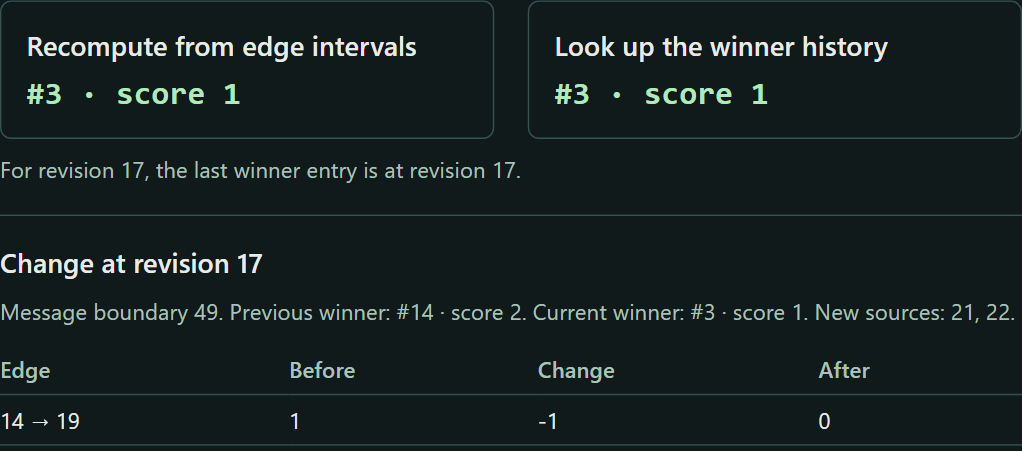
\includegraphics[width=.99\columnwidth]{withdrawal.png}
\caption{Companion SQLite console for a historical source withdrawal. A visitor can move the requested revision independently of the committed horizon and inspect the two read plans. This console uses a tool trace. The Git replay in Table~\ref{tab:demo} uses co-edits.}
\label{fig:trace}
\end{figure}

\subsection{Withdraw a source and rewind}
In the companion console (Fig.~\ref{fig:trace}), advance trace q11 to revision 17 and request revision 16. Producer 14 leads with score 2, ahead of producer 3 with score 1. Advance the read revision to 17. The named edge from producer 14 to consumer 19 changes from 1 to 0. Producer 3 now wins the tie. Rewinding the read returns producer 14. The console compares an interval query over active supports with a journal that writes only changes in the winning pair. It illustrates the role of the tie rule and the difference between an observed withdrawal and an evicted but still valid Git event. On 40 ISETrace trajectories~\cite{ise}, the two plans agreed across 1,112 historical states. Incremental top-$k$ views offer another way to reduce refills when maintaining a global ranking~\cite{topk}. Here each Git query supplies a new anchor and requires a conditional ranking.

\section{Evaluation}
\subsection{Information quality at a fixed retention policy}
We replayed four panels (Table~\ref{tab:recall}). A query reveals one path in a multi-file commit and asks for eight companions. All judgments use the unobserved remainder of that commit. Recall@8 is the fraction of those paths recovered, averaged by query. Previously unseen targets remain in the denominator. We rank before inserting the target commit. The long panel comprises 4,096 consecutive first-parent transitions each for NetworkX, Matplotlib and Sphinx. In the second half of each history a deterministic SHA rule selects eligible commits and the anchor. An independent audit compared all 12,288 deltas to the raw parent and child Git trees. Rename inference is disabled. A path that moves acquires a new identity. The other panels reuse earlier research histories and provide checks on how results vary across projects.

\begin{table}[t]
\caption{Git companion-file Recall@8 (\%). All policies see the same prefix for each query. Small decodes the eight smallest eligible events, with additional metadata reads.}
\label{tab:recall}\centering\small
\begin{tabular}{@{}lrrrrr@{}}\toprule
Panel & Queries & Own & Shared & Small & Full\\\midrule
A & 1,075 & 58.44 & 58.24 & 59.71 & 58.84\\
B & 880 & 48.13 & 48.49 & 48.94 & 48.83\\
C & 1,216 & 50.45 & 51.99 & 51.71 & 52.20\\
Long & 196 & 41.97 & 43.53 & 45.88 & 46.33\\\bottomrule
\end{tabular}
\end{table}

Our prespecified long-panel contrast improved 15 queries, degraded 12 and tied on 169. The pooled change was $+1.56$ percentage points (pp). The changes were $+4.63$ pp for Matplotlib, $-0.17$ for NetworkX and $+0.42$ for Sphinx. Three projects support a descriptive comparison. Sharing raised the number of event bodies decoded from 1,258 to 4,988. Reading the smallest eligible events produced 45.88\%. A subsequent control based on transaction-size filtering~\cite{moonen} reached 47.32\%. Giving events of size at most six priority, filling unused slots by recency and weighting each vote by $1/(|M_e|-1)$ reached 48.90\% in a post hoc comparison. This result motivates replication of the size heuristic.

Agreement with the full-history ranking measures a different outcome. Without archive reads, the own and shared outputs, including exact scores, matched on 604/880 (68.64\%) and 714/880 (81.14\%) of B. They matched on 66/196 (33.67\%) and 82/196 (41.84\%) of long. Checking the count bounds certified 740/880 (84.09\%) and 81/196 (41.33\%) without a lookup. A visible answer can coincide with the oracle even when its exactness cannot be proved from the summaries. With the archive enabled, all 1,076 exact responses on these two panels matched the oracle.

\subsection{What does an exact read cost?}
Table~\ref{tab:reads} measures the SQLite boundary in a warm local write-ahead-log configuration. Both cached readers use the same choice of live event bodies. Own-window recovery asks for the older prefix. Shared recovery asks for fully evicted incidents. The full packed baseline gets all anchor events in one query. Additional controls on the long panel took 14.21\,ms for a materialized pair table, 28.79\,ms for SQL grouping and 33.47\,ms for an in-memory bitset reader scanning candidates. All answers use exactly the same ordered IDs and counts. Times include constructing each result but exclude common metadata preparation and writes. Event payload bytes transferred to the client measure logical work at the API boundary.

\begin{table}[t]
\caption{Exact reads. Each time is the median of five totals over an entire panel in milliseconds. The byte column counts the event payload returned by SQLite.}
\label{tab:reads}\centering\small
\setlength{\tabcolsep}{4pt}\begin{tabular}{@{}llrrrr@{}}\toprule
Panel & Plan & SQL calls & Events & Bytes & ms\\\midrule
B & Full packed & 880 & 7,141 & 204,088 & 19.38\\
& Own + archive & 281 & 3,094 & 74,840 & 14.76\\
& Shared + archive & 172 & 687 & 8,076 & 12.86\\\midrule
Long & Full packed & 196 & 7,034 & 358,964 & 16.83\\
& Own + archive & 130 & 5,776 & 296,332 & 15.71\\
& Shared + archive & 115 & 2,046 & 27,716 & 12.92\\\bottomrule
\end{tabular}
\end{table}

Durable costs include work on the write path. On fresh databases, with one FULL-synchronous WAL transaction per accepted event and one read per sampled decision, the median total write-plus-read time over three randomized blocks was 2.429\,s for full packed and 2.376\,s for shared on long. The sum of checkpointed database sizes was 664 versus 500\,KiB. Reopening took 4.87 versus 15.45\,ms. Shared restored 3,320 live events and 600 cold-file IDs. On B the packed and shared plans took 465.4 and 473.0\,ms and occupied 196 and 200\,KiB, respectively. Writes dominated the mixed workload. The counts of bytes transferred by reads alone cannot predict footprint, restart time or end-to-end speed.

\subsection{Transfer to a published coding benchmark}
Agent Retrieval Bench~\cite{arb} supplies repository snapshots and lists of required files. On its \emph{code2test} task, known implementation paths may be used to select related tests. The published Recall@5 values for seven released rankings were reproduced on all 106 canonical tasks. For our paired transfer test, 105 eligible tasks from 12 repositories inherited the earlier panel's inclusion rule. Both policies may return five new paths. The control filters Qwen3-Embedding-4B's published ranks by test role and fills from path-name similarity. The challenger preserves the first four results and conditionally replaces the fifth using prior co-edits in 64 first-parent transitions. This is a separate history-based retrieval policy. It does not exercise the exact SQLite reader.

Mean Recall@5 changed from 68.98\% to 69.62\%, a paired difference of $+0.63$ pp before rounding (repository bootstrap 95\% interval $[-2.58,+3.30]$, four wins, two losses and 99 ties). An exploratory five-source rank ensemble gained 2.98 pp when adding historical votes, while including a further strong static retriever reduced the marginal gain to 0.48 pp. All 105 queries had been used in earlier work under a different task formulation. These observations do not establish a benchmark lead. In a separate pilot on 36 masked functions, a local Qwen3-4B-Instruct-2507 solver passed all example tests for 15 functions using recent co-edited tests and for 15 with full-history BM25. The accuracy evidence concerns file discovery and small executable examples. A benefit for autonomous issue resolution remains open.

\section*{Acknowledgments}
OpenAI Codex drafted Sections I--IV, implemented and exercised the prototypes, produced the figures, and analyzed the stored rankings and measurements. The artifact includes the per-query outputs, pinned inputs, protocols and independent checks for the reported comparisons.

\balance
\bibliographystyle{IEEEtran}
\bibliography{sources}
\end{document}
